
% This .tex file (and associated .cls) produces:
%       1) The Permission Statement
%       2) The Conference (location) Info information
%       3) The Copyright Line TSConIT
%       4) NO page numbers
%       5) NO headers and/or footers
%
% Using 'sig-alternate.cls' you have control, however, from within
% the source .tex file, over both the CopyrightYear
% (defaulted to 200X) and the ACM Copyright Data
% (defaulted to X-XXXXX-XX-X/XX/XX).
% e.g.
% \CopyrightYear{2007} will cause 2007 to appear in the copyright line.
% \crdata{0-12345-67-8/90/12} will cause 0-12345-67-8/90/12 to appear in the copyright line.
%
% ---------------------------------------------------------------------------------------------------------------
% This .tex source is an example which *does* use
% the .bib file (from which the .bbl file % is produced).
% REMEMBER HOWEVER: After having produced the .bbl file,
% and prior to final submission, you *NEED* to 'insert'
% your .bbl file into your source .tex file so as to provide
% ONE 'self-contained' source file.
%

% refers to the cls file being used
\documentclass{sig-alternate-br}
\usepackage{float}
\usepackage{caption}
\usepackage{subcaption}
\usepackage{hyperref}

\restylefloat{figure}
\restylefloat{table}
\begin{document}

%
% --- Author Metadata here --- DO NOT REMOVE OR CHANGE 
%\conferenceinfo{13$^{th}$ Twente Student Conference on IT}{June 23$^{st}$, 2010, Enschede, The Netherlands.}
\CopyrightYear{2015} % Allows default copyright year (200X) to be over-ridden - IF NEED BE.
%\crdata{0-12345-67-8/90/01}  % Allows default copyright data (0-89791-88-6/97/05) to be over-ridden - IF NEED BE.
% --- End of Author Metadata ---

\title{micro data server using raspberry pi}
% In Bachelor Referaat at University of Twente the use of a subtitle is discouraged.
 \subtitle{Research Proposal}




\numberofauthors{1} 
\author{ 
% You can go ahead and credit any number of authors here,
% e.g. one 'row of three' or two rows (consisting of one row of three
% and a second row of one, two or three).
%
% The command \alignauthor (no curly braces needed) should
% precede each author name, affiliation/snail-mail address and
% e-mail address. Additionally, tag each line of
% affiliation/address with \affaddr, and tag the
% e-mail address with \email.
%
% 1st. author
\alignauthor P.j.e. Velthuis\\
       \affaddr{University of Twente}\\
       \affaddr{P.O. Box 217, 7500AE Enschede}\\
       \affaddr{The Netherlands}\\
       \email{p.j.e.velthuis@student.utwente.nl}
% 2nd. author
\alignauthor 2nd Author\\
       \affaddr{2nd author's affiliation}\\
       \affaddr{1st line of address}\\
       \affaddr{2nd line of address}\\
       \email{2nd author's email address}
% 3rd. author
\alignauthor 3rd Author\\
       \affaddr{3rd author's affiliation}\\
       \affaddr{1st line of address}\\
       \affaddr{2nd line of address}\\
       \email{3rd author's email address}
}

%\additionalauthors{Additional authors: John Smith (The
%Th{\o}rv{\"a}ld Group, email: {\texttt{jsmith@affiliation.org}})
%and Julius P.~Kumquat (The Kumquat Consortium, email:
%{\texttt{jpkumquat@consortium.net}}).}
%\date{30 July 1999}


\maketitle
\begin{abstract}
This paper describes the performance of raspberry pi load balancing service using video streaming.
\end{abstract}

\keywords{Cloud computing, Raspberry Pi,  micro data server, video streaming, load balancing}

\section{Introduction}
Today cloud computing becomes more important. The amount of cloud computing services is increasing fast \cite{armbrust:2009}.  Despite the attention from the research community, research and development of Cloud Computing services is still in it's childhood~\cite{tso:2013}. 
Cloud computing is a trend IT that people move computing and data away from desktop and portable PCs into large data centers~\cite{dikaiakos:2009}. People will in the future access internet services over lightweight portable devices. In this research the Raspberry Pi cloud services will be investigated. A reason for this is that the density of servers has increased a lot in the past~\cite{density}. There are new technologies such as for example the ARM processor. Many companies want to explore the possibilities of for example the Raspberry Pi and his ARM Processor. Some data centers even offer some cloud computing using the Raspberry Pi. A reason for this is the small location that the Raspberry Pi needs, and the low power usage of a Raspberry Pi\cite{hosting,Pcextreme}.  A Raspberry Pi has a power usage between the 3-5 Watt. A normal server has a power usage between the 75 and 250 watt \cite{Powerusage,beloglazov2012energy}. This could mean that it is better to use a Raspberry Pi for specific small tasks that do not demand a whole server. During this research there will be a investigation on the performance of the Raspberry pi as a server.  A Raspberry Pi can be the small data center for the future \cite{tso:2013}. The Raspberry is a rather cheap device for 35 euros. This makes it cheaper to do research in compared to a normal server. This is also the mean reason why the Raspberry pi was ones created. The current versions of the Raspberry Pi cannot perform the task of a large scale x86 server \cite{tso:2013}. Building a cloud like this can be a cost effective scale model\cite{tso:2013}. It's a ideal testbed for testing distributed software. During this research we will investigate the performance of a raspberry pi as a video streamer to other computers. The reason I want to investigate it with video streaming is because this demands a lot of bandwidth from the network and could be one of the first things that should be improved. 

Today a lot of people watch their movies online using video streaming. The Netherlands have for example one million subscribers for Netflix \cite{volkskrant}. Netflix is a video streaming service that makes HD movies watching possible. For this Netflix makes use of a content distribution network (CDN). On the internet this is also known as a on demand service \cite{Adhikari:2012}. Netflix makes use of MPEG-DASH a protocol that makes streaming over http possible \cite{martin:2013}. The problem is that Netflix is responsible for  29.7\% of the peak downstream traffic in US  \cite{Adhikari:2012}. In the Netherlands more and more users are making use of video streaming as Youtube and Netflix. In this research there will be a investigation on the possibility to make small micro data centers with raspberry pi's. This research will try to find out how this cloud works. There will be taken a look in for example the load balancing of video streaming. In this way it can be possible to see improvements that can be made in the load balancing so that the servers can be used more efficient. This is also build to learn more from load balancing and a computer cluster. This can be really useful, because nowadays it's still done on relatively expensive servers. 

In this paper we will try to measure the performance of different load balancing techniques using the Raspberry Pi. For this the main research question will be: 
\begin{center}
 What is the performance of a raspberry pi load balancing techniques using video streaming?
\end{center}

In order to come to a good answer we need to  research several things. Therefore several sub-questions will be researched. These sub-questions will altogether provide a answer to the main research question. 

\begin{enumerate}
	\item What is small scale cloud computing?
	\item What is cloud video streaming?
	\item What kind of different load balancing techniques are there?
	\item Is it reachable to build small personal Raspberry Pi clouds for services?
	\item Is it possible to improve load balancing using small scale Raspberry Pi's? 
\end{enumerate}

This research will be part literature study and a part of it will be building a small Raspberry Pi cloud to analyze balancing techniques on the Raspberry Pi. For this research cloud video streaming is one of the specific aspects that will be investigated. The load balancing techniques will be optimized for the video streaming. The first three research questions will describe the state of the art. 
The last two sub-questions will go into the technical research that will investigate the performance and possibility of Raspberry Pi's for cloud video streaming. They last one will investigate of their are improvements in load balancing possible. The five sub-questions are being looked at in the next five sections. Followed by a final section for conclusions and identified areas for future
work.


\section{Small scale computing}
Today there are many cloud kinds of cloud computing. The amount of cloud computing services is increasing fast \cite{armbrust:2009}. It's now even possible to build your own small cloud using Raspberry Pi's \cite{southampton,abrahamsson:2013}. In this research there will be small scale cloud computing with the Raspberry Pi. The main motivation behind this is that it is ways to expensive to simulate large scale cloud computing. Another reason is the small location that is needed used with small scale cloud computing for Raspberry Pi's\cite{Pcextreme}. The Raspberry Pi is really small compared to a normal server \cite{cox:2014}. Because of this it could be better in executing small tasks. Small scale cloud computing is cloud computing with smaller computation amounts than normal \cite{cox:2014}. More motivation is that it does not use a lot cooling and power \cite{tso:2013}.  Most clients of cloud computing buy the services instead of the hardware and having to set up the servers themselves. 
The Amazon Elastic Compute Cloud (Amazon EC2) is one of the most widely used infrastructure platforms that these clients use \cite{hofer:2011}. This elasticity of computing resources is very important~\cite{Miettinen:2010:EEM:1863103.1863107}. 

\subsection{What is it?}
To understand what small scale cloud computing really is we will look more at the specific cloud service called Infrastructure as a Service. To this specific cloud service belongs the online storage. Today a lot of companies have their own virtual machines running in large data centers \cite{beloglazov:2010}. These instances can most often be scaled dynamically to the customer it's need. Using these instances makes it easier management and varying workloads better possible. The Raspberry Pi is a lot cheaper and has less power consumption, because of this it can be interesting 
to host virtual machines on the Raspberry Pi. The reason we call it small scale is because it is using small Raspberry's instead of large servers. Some providers offer a special hybrid cloud. You can then connect a private cloud to a public cloud \cite{qian:2009}. 


\subsection{Storage}
In the cloud there are several storage systems.  The cloud storage has become an integral part of our modern and mobile lives. Nowadays people own more often multiple devices. Cloud storage made it possible that the files we need are available where and when we want them. There are several ways to do this storage. Dropbox for example stores your information on a local folder on your device, after it has done that it will sync with an online version \cite{drago2012inside, dropbox}. In this way your other devices or the friends you shared the information with will have that information. In this way offline editing is also possible and this makes dropbox really powerful. \newline
Today there are a lot of problems with security for cloud storage and that's why some people like to do it by themselves. For this there is a cloud service called ownCloud \cite{owncloud}. This service gives you the possibility to host the data where you want. You can even build your own cloud storage system by using ownCloud open source. The security aspect is important, because this can lead to loss or leak of data. Sometimes this can even have legal consequences \cite{hofer:2011}. For all important software used for cloud storage this means that they should be stored server side \cite{hofer:2011}. \newline
Another problem that is very important is the reachability of the data centers that are used by the cloud. Netflix responsible for 29.7\% of the peak downstream traffic in US  \cite{Adhikari:2012}.

\subsection{Power usage}
Power usage efficiency is nowadays becoming a more important aspect in cloud computing. This is one of the main problems in cloud computing. Data centers require a lot of electrical power. Therefore we perhaps need to more Green Cloud Computing solutions that reduce the electrical power consumption and reduce the environmental impact of data centers~\cite{beloglazov2012energy}. Besides the power the data center consumes it can be important to look at the traffic pattern. It can make a huge different in sending data in small bursts or in one large burst \cite{Miettinen:2010:EEM:1863103.1863107}. With the increase of lightweight portable devices the energy efficiency becomes more important. This means that a trade-of has to be made between local processing and computation offloading \cite{Miettinen:2010:EEM:1863103.1863107}. This is computation offloading makes cloud computing more and more important. 

\section{Video streaming}
There are a lot of cloud services nowadays. These include a webserver, a DNS server, a chat server, a mail server, a vpn server or a monitoring server or even a video streaming service. \newline
Today a lot of people watch their movies online using video streaming and this amount of people is increasing. The netherlands have for example one million subscribers for Netflix \cite{volkskrant}. One thing that these users want is the on demand video streaming. They don't want to store the data itself and they want to have a wide choice of different videos. Netflix is a video streaming service that makes HD movies watching possible. For this Netflix makes use of a content distribution network (CDN). On the internet this is also known as a on demand service. They make use of amazon its AWS, Amazon simpleDB , S3 and cassandra for file storage \cite{Adhikari:2012}. Netflix makes use of MPEG-DASH a protocol that makes streaming over http possible. Currently Netflix has 30\% of the downstream in the United States~\cite{computer-networking}. To make this video streaming possible Netflix does some things in the cloud. These are content ingestion, content processing and uploading different versions to the CDN (Content Distribution Networks)~\cite{Adhikari:2012}. Content ingestion means that Netflix receives the studio master version of the movies and uploads these to the cloud. In the cloud there are then created many different formats for each movie. Once all these versions have been created they are distributed over the multiple CDNS. 

The video streaming happens with TCP. TCP sends frames to the client and in these frames is the video stored. Of course if the available TCP send rate is large enough then the video will play without any delays. But if the TCP send rate is less then needed then the video play will alternate between periods of continuous playout and periods of freezing~\cite{computer-networking}. Its very important that video freezing or audio playing faster then the video does not happen. This is why multimedia applications have high performance requirements. For this their are models to predict the performance and techniques to find a minimal cost bandwidth allocation that will result in all user requirements being met. 

\subsection{HTTP streaming}
HTTP streaming is one way to stream a video. In HTTP streaming the HTTP GET request specifies the specific range of bytes the client wants to retrieve from the desired video~\cite{computer-networking}. In this way the client can correctly receive the video. If the client receives to much then its buffer for video playing can get full. To prevent throwing data away the server will then stop sending. To prevent throwing data away the client will have a not to large buffer. \newline
There is also a new kind of HTTP streaming called DASH (Dynamic Adaptive Streaming over HTTP)~\cite{computer-networking}. In DASH the video is encoded into several different versions. If the bandwidth is high, then the client selects chunks from a high-rate version and the way around~\cite{computer-networking}. The possibility to switch between bit rate versions is in video streaming very important. To make a smooth transition between these versions possible there are intermediate versions so that the client will see less suddenly the change in video quality. In HTTP streaming the server stores the video with a different URL.   

To investigate video streaming there will be an experimentation cloud with Raspberry Pi's to see if these small mini computers will work as a cloud. 
Resources I could use for cloud video streaming:
\cite{g-streamer,raspberry-video,video-1080p, plissonneau:2012}
 
\section{Load balancing}
In distributed servers it is very important that good load balancing takes place. There are several choices that have to be made by choosing a load balancer for a service. These choices can for example be performance, reliability and features.There are several load balancing techniques out there, for example priority queuing~\cite{computer-networking}. This means that packets in the output queue are prioritized. This is typically done in a first in first out way. Another type of queuing is the round robin. Round robin puts packets into different classes. It will first look for a packet in a given class and if there is none in that class it will look for the next packet \cite{computer-networking}. A more abstract form of round robin is weighted fair queuing. The difference between these is that each class may receive a differential amount of service in any interval of time \cite{computer-networking}.  
\subsection{Video streaming and load balancing}
For video streaming several load balancing techniques can be used. There can be a non-uniform demand for different movies. One solution to overcome this problem would be to replicate the most popular movies. One obvious problem is then that it is expensive in terms of storage space required. To solve this you can use dynamic replication to solve the load demand~\cite{dan1996load}. By using this you move portions of a movie to less used storage devices. The allocation of these movies only happen when there is a to high increase on one specific storage device. In this way load imbalances can be prevented \cite{dan1996load}. \newline
Load balancers are generally grouped in two layers. Layer 4 (FTP,IP, UDP, TCP )and layer 7 the application layer. Layer 7 load balancers distribute request based upon data in the application layer, this can for example be HTTP. A lot of video streaming services use http streaming \cite{Adhikari:2012}. 

\cite{wolf:1997,load-balancing}


\section{Research Methods}
This research will investigate a cloud computer consisting of Raspberry Pi's. The research method for this would be the Design Science research method. this is a method to solve field problems. This research will make use of the design Science method proposed by Hevner~\cite{hevner:2007}. This design method has three variants. 
\begin{figure}[H]
	\centering 
	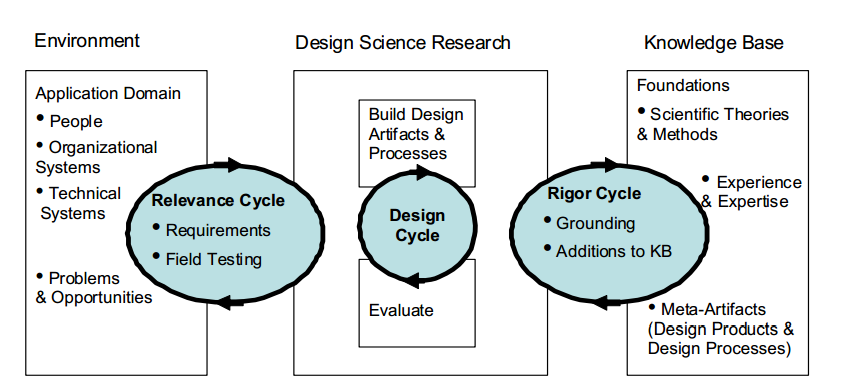
\includegraphics[width=0.4\textwidth]{Design_science.png}
	\caption{Design Science}
	\label{fig:design} %always place your label after your caption!
\end{figure}
The \textbf{relevance cycle} is important, because you first have to identify the problems and opportunities. The \textbf{design cycle} is where you actually build the design. The \textbf{rigor cycle} matters because it can give you two types of additional knowledge. It provides past knowledge to ensure its invention and it's there to guarantee that the now product is a research contribution.

\section{Research approach}
For the experiment we need a Raspberry Pi with a static Ip address and we need a sd card for the OS. For the experiment we need a Raspberry Pi B that can make use of the Ethernet. This is because a Raspberry Pi can be used as a webserver and this is needed to have this in order to make video streaming possible. This webserver will make video streaming possible. It will have a VPN to make it possible to put video's on the Raspberry pi \cite{VPN:2014}. 
So I will first make this video streaming webserver. 
After this we will make a cluster with one Raspberry Pi as a load balancer and the other two as a video stream pi. If I have made such I cluster I can start doing some tests on it. For example some test in streaming in different quality with load balancing. The setup of the raspberry Pi can be seen in the figure below ~\ref{fig:setup}.

\begin{figure}[H]
\centering 
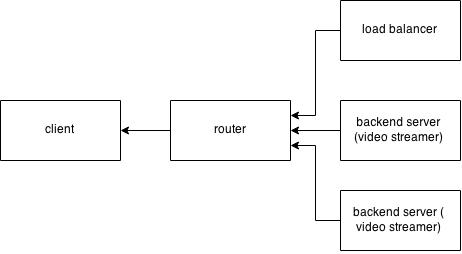
\includegraphics[width=0.4\textwidth]{raspberry pi setup.jpg}
\caption{Raspberry Setup}
\label{fig:setup} %always place your label after your caption!
\end{figure}
For the load balancing we will make use of Nginx for this we will use the following sources:
\cite{nginx-load-balancing, nginx-load-balancing-2}

\section{Raspberry pi}
\begin{figure}[H]
\centering 
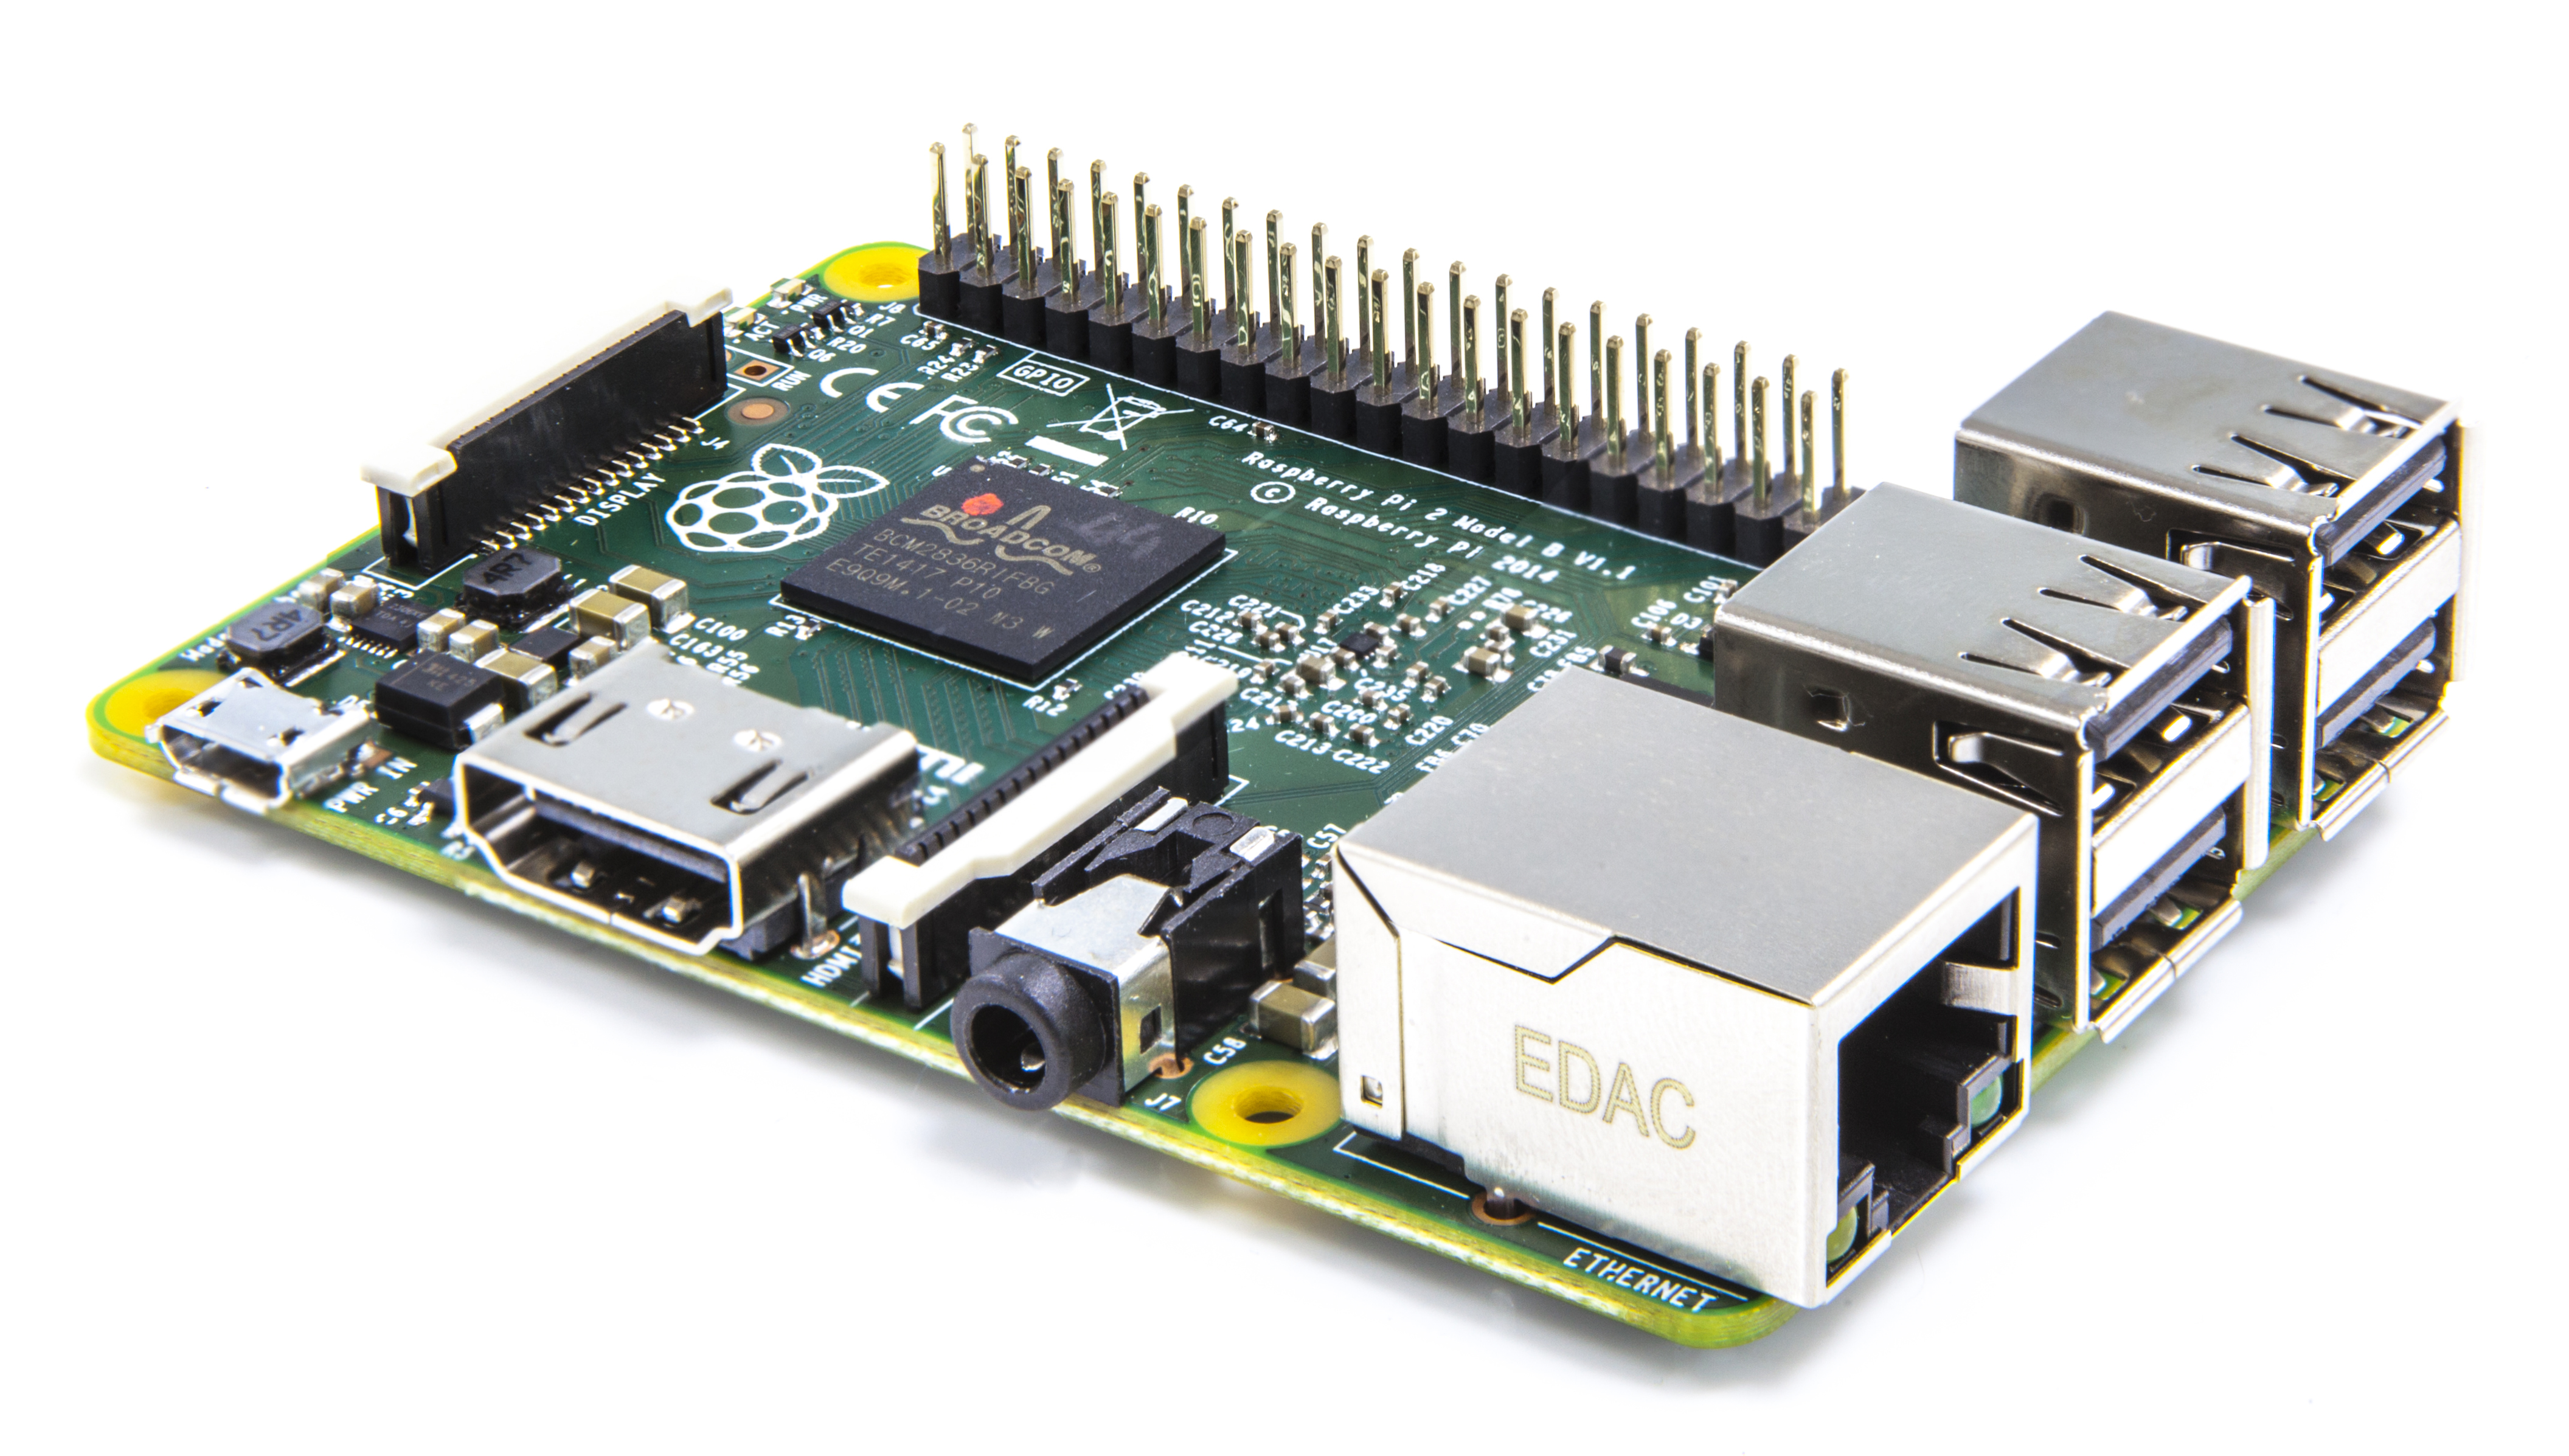
\includegraphics[width=0.4\textwidth]{Pi2ModB1GB_-comp.jpeg}
\caption{Raspberry Pi 2 model B}
\label{fig:raspberry} %always place your label after your caption!
\end{figure}
\begin{table}[H]
	\centering \caption{Specificaties}
	\begin{tabular}{|c|c|} \hline
		Ethernet & 100 MBps \\ \hline
		USB & 4 x USB 2.0 \\ \hline
		Video out & HDMI 1.4 \\ \hline
		Audio & 2 x analog \\ \hline
		CPU & 900MHz quad-core ARM Cortex-A7 \\ \hline
		card slot & Micro SD  \\ \hline
	\end{tabular}
		\label{tab:Specificaties}
\end{table}
The Raspberry Pi only consumes 3 watts, because of this it doesn't need active cooling. 
With this subquestion I want to find out if it is possible to let users have small Raspberry Pi servers I also want to know what the performance of this small Raspberry Pi cloud is. 
Resources:
\cite{Pcextreme,nginx-load-balancing,nginx-load-balancing-2}

For this research I want to investigate if it is possible to do more research in the 
load balancing techniques that can be used in a raspberry pi. A example of this would be the round robin queuing~\cite{nginx-load-balancing,nginx-load-balancing-2}.

\subsection{Raspberry Pi cloud projects}
there have been several cloud projects with the raspberry Pi. \newline
One of these has been the supercomputer build by Southampton~\cite{cox:2014}. Here they build it with 64 raspberry Pi's . They used a Message Passing interface to communicate between the raspberry pi's. The research was done in order to see what the performance of a low-power high performance cluster is. \newline
The project of the university of Glasgow~\cite{tso:2013}. This data center has 56 Raspberry Pi's. It is build for research and education purposes for a cloud data center. They have a hadoop running on their servers. \newline
There was another project called the Beowulf cluster~\cite{beowolf-setup}. This project was created for a phd assignment. This cluster is build for collaboratively processing sensor data.  A Beowulf cluster is simply a collection
of identical, (typically) commodity computer hardware based systems~\cite{beowolf-setup}. The big advantage of the Raspberry Pi in this project was that it is cheap and it does not need a cluster administrator to watch over everything you do. 

\section{State of the Art}
 People want to have everything has to be accessible through the network around the clock \cite{youseff:2008}. One thing that people want on demand are there film series. Currently Netflix has 30\% of the downstream in the United States. This downstream is huge and that means that there is optimization in this branch possible. To make the video on demand service of Netflix possible they use servers from Amazon. 

In this paper there will be research done on making a load balancing service for the Raspberry Pi.  This service will consist of several raspberry Pi's. These Raspberry Pi's make together a small cloud computer.  The Raspberry Pi is made for research and education purposes \cite{raspberry-pi}. The Raspberry Pi is a cheap device costing around 35 euro. It has a power consumption of only three watt and has quite good processor. For this reason it might be very useful for small scale cloud computing. The raspberry Pi is a small device and is excellent for a lot of small devices in a relatively small place. The Raspberry Pi doesn't use cooling and it can be used for very rapid elasticity and on-demand self-service. Because of it's cooling features and low power consumption it might be a good alternative for the nowadays high power consuming data centers. The raspberry pi is really small so it is a lot easier to place extra pi in a data center compared to a normal server. The Raspberry Pi has one drawback and that is that the processing power is relatively low. By using load balancing there will be taken a look at what load balancing techniques are successful for the Raspberry pi. 

In this research we will make a small raspberry cloud to do research on video streaming using HTTP. This will be done using the design Science method proposed by Hevner\cite{hevner:2007}. After we have done this for the Raspberry Pi there will be looked at streaming using Amazon. In this way we can see how the results are compared to streaming via Amazon. This research will try to find out if the raspberry has enough processing power to stream to multiple web clients. The cloud performance can now be better researched, because everything is at one location and the information about what processes are running on the pi are well defined. In this way we can take a better look at algorithms used in video streaming. This is mostly because there is not a lot of overhead. 

\section{Conclusion and future work}

\section{Acknowledgments}
This paper would not have been possible without the help of Björn Postema and Nick Shot.

\bibliographystyle{abbrv}
\bibliography{sigproc}  % sigproc.bib is the name of the Bibliography in this case
% You must have a proper ".bib" file
%  and remember to run:
% latex bibtex latex latex
% to resolve all references
%
% ACM needs 'a single self-contained file'!
%
\vspace{50 mm}
\newpage
%APPENDICES are optional


\end{document}
